\documentclass{article} 
\usepackage[utf8]{inputenc} 
\usepackage[spanish]{babel}
\usepackage{graphicx}

\title{Cuestionario - Primer Interciclo\\Introducción a Big Data}
\author{Recurso Docente - ISTA}
\date{\today}

\begin{document}

    \maketitle

    \begin{enumerate}
        \item En el flujo de proceso de gestión BigData, arrastre los elementos al lugar que corresponde:
            \begin{figure}[!h]
                \centering
                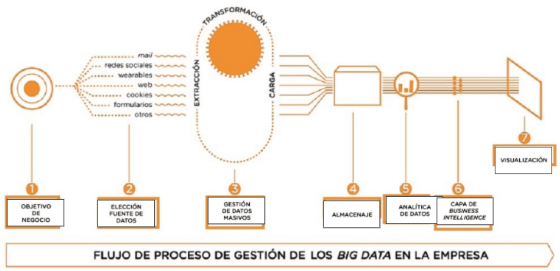
\includegraphics[width=0.9\textwidth]{img/recurso-1.png} 
            \end{figure}
        
        \item Con el paso del tiempo las empresas han fomentado la creación de \underline{estrategias} para la toma de \underline{decisiones}, dando un importante lugar al análisis \underline{predictivo}, ya que con esto se han podido determinar diversos tipos de \underline{patrones} entre la sociedad, generando como consecuencia gran cantidad de \underline{beneficios} consistentes en la innovación, investigación y desarrollo de nuevas \underline{soluciones}.
        \item Relacione la definición con su concepto:
            \begin{itemize}
                \item Tasa de datos. [Velocidad]
                \item Cantidad generada de datos. [Volúmen]
                \item Presición del dato. [Veracidad]
                \item Cantidad de fuentes de datos. [Variedad]
                \item Su valor cambia con el tiempo. [Variabilidad]
                \item Transformar/Extraer. [Valor]
                \item Datos sintetizados. [Visualización]
            \end{itemize}
        
        \item Relaciona el concepto con el autor correspondiente. El BigData es:
            \begin{enumerate}
                \item 
            \end{enumerate}
        
        \item 
    \end{enumerate}

\end{document}